\let\negmedspace\undefined
\let\negthickspace\undefined
\documentclass[journal]{IEEEtran}
\usepackage[a5paper, margin=10mm, onecolumn]{geometry}
%\usepackage{lmodern} % Ensure lmodern is loaded for pdflatex
\usepackage{tfrupee} % Include tfrupee package

\setlength{\headheight}{1cm} % Set the height of the header box
\setlength{\headsep}{0mm}     % Set the distance between the header box and the top of the text

\usepackage{gvv-book}
\usepackage{gvv}
\usepackage{cite}
\usepackage{amsmath,amssymb,amsfonts,amsthm}
\usepackage{algorithmic}
\usepackage{graphicx}
\usepackage{textcomp}
\usepackage{xcolor}
\usepackage{txfonts}
\usepackage{listings}
\usepackage{enumitem}
\usepackage{mathtools}
\usepackage{gensymb}
\usepackage{comment}
\usepackage[breaklinks=true]{hyperref}
\usepackage{tkz-euclide} 
\usepackage{listings}
% \usepackage{gvv}                                        
\def\inputGnumericTable{}                                 
\usepackage[latin1]{inputenc}                                
\usepackage{color}                                            
\usepackage{array}                                            
\usepackage{longtable}                                       
\usepackage{calc}                                             
\usepackage{multirow}                                         
\usepackage{hhline}                                           
\usepackage{ifthen}                                           
\usepackage{lscape}
\usepackage{circuitikz}
\tikzstyle{block} = [rectangle, draw, fill=blue!20, 
    text width=4em, text centered, rounded corners, minimum height=3em]
\tikzstyle{sum} = [draw, fill=blue!10, circle, minimum size=1cm, node distance=1.5cm]
\tikzstyle{input} = [coordinate]
\tikzstyle{output} = [coordinate]


\begin{document}

\bibliographystyle{IEEEtran}
\vspace{3cm}

\title{4.4.33}
\author{AI25BTECH11037-stalin}
 \maketitle
% \newpage
% \bigskip
{\let\newpage\relax\maketitle}
\renewcommand{\thefigure}{\theenumi}
\renewcommand{\thetable}{\theenumi}
\setlength{\intextsep}{10pt} % Space between text and floats
\numberwithin{equation}{enumi}
\numberwithin{figure}{enumi}
\renewcommand{\thetable}{\theenumi}
\textbf{Question}:\\
\text{Find the value of } x \text{ such that the four points with position vectors } $\vec{A}(3\hat{i} + 2\hat{j} + \hat{k}), \vec{B}(4\hat{i} + x\hat{j} + 5\hat{k}), \vec{C}(4\hat{i} + 2\hat{j} - 2\hat{k}), \text{ and } \vec{D}(6\hat{i} + 5\hat{j} - \hat{k})$ \text{ are coplanar.} \quad (12, 2018)
\\
\solution \\
Let us solve the given equation theoretically and then verify the solution computationally \\
According to the question, \\
Given four position vectors\\
\begin{align}
    \vec{A}=\begin{myvec}{3\\2\\1}\end{myvec}\
    \vec{B}=\begin{myvec}{4\\x\\5}\end{myvec}\
    \vec{C}=\begin{myvec}{4\\2\\-2}\end{myvec}\
    \vec{D}=\begin{myvec}{6\\5\\-1}\end{myvec}\
\end{align}
\begin{align}
    \vec{A}^T\vec{n}=1
\end{align}
\begin{align}
    \vec{B}^T\vec{n}=1
\end{align}
\begin{align}
    \vec{C}^T\vec{n}=1
\end{align}
\begin{align}
    \vec{D}^T\vec{n}=1
\end{align}
\begin{align}
    \begin{myvec}{A&&B&&C&&D}^T\end{myvec}\vec{n}=\begin{myvec}{1\\1\\1\\1}\end{myvec}
\end{align}
Let 
\begin{align}
    \vec{i}=\myvec{1\\1\\1\\1}\
    \vec{z}=\begin{myvec}{A&&B&&C&&D}^T\end{myvec}
\end{align}
condition is Rank of $\begin{myvec}{A&&B&&C&&D}^T\end{myvec}$=3
and $\begin{myvec}{z&&i}\end{myvec}$=3\\
From solving we get x=5.

\begin{figure}[h!]
    \centering
    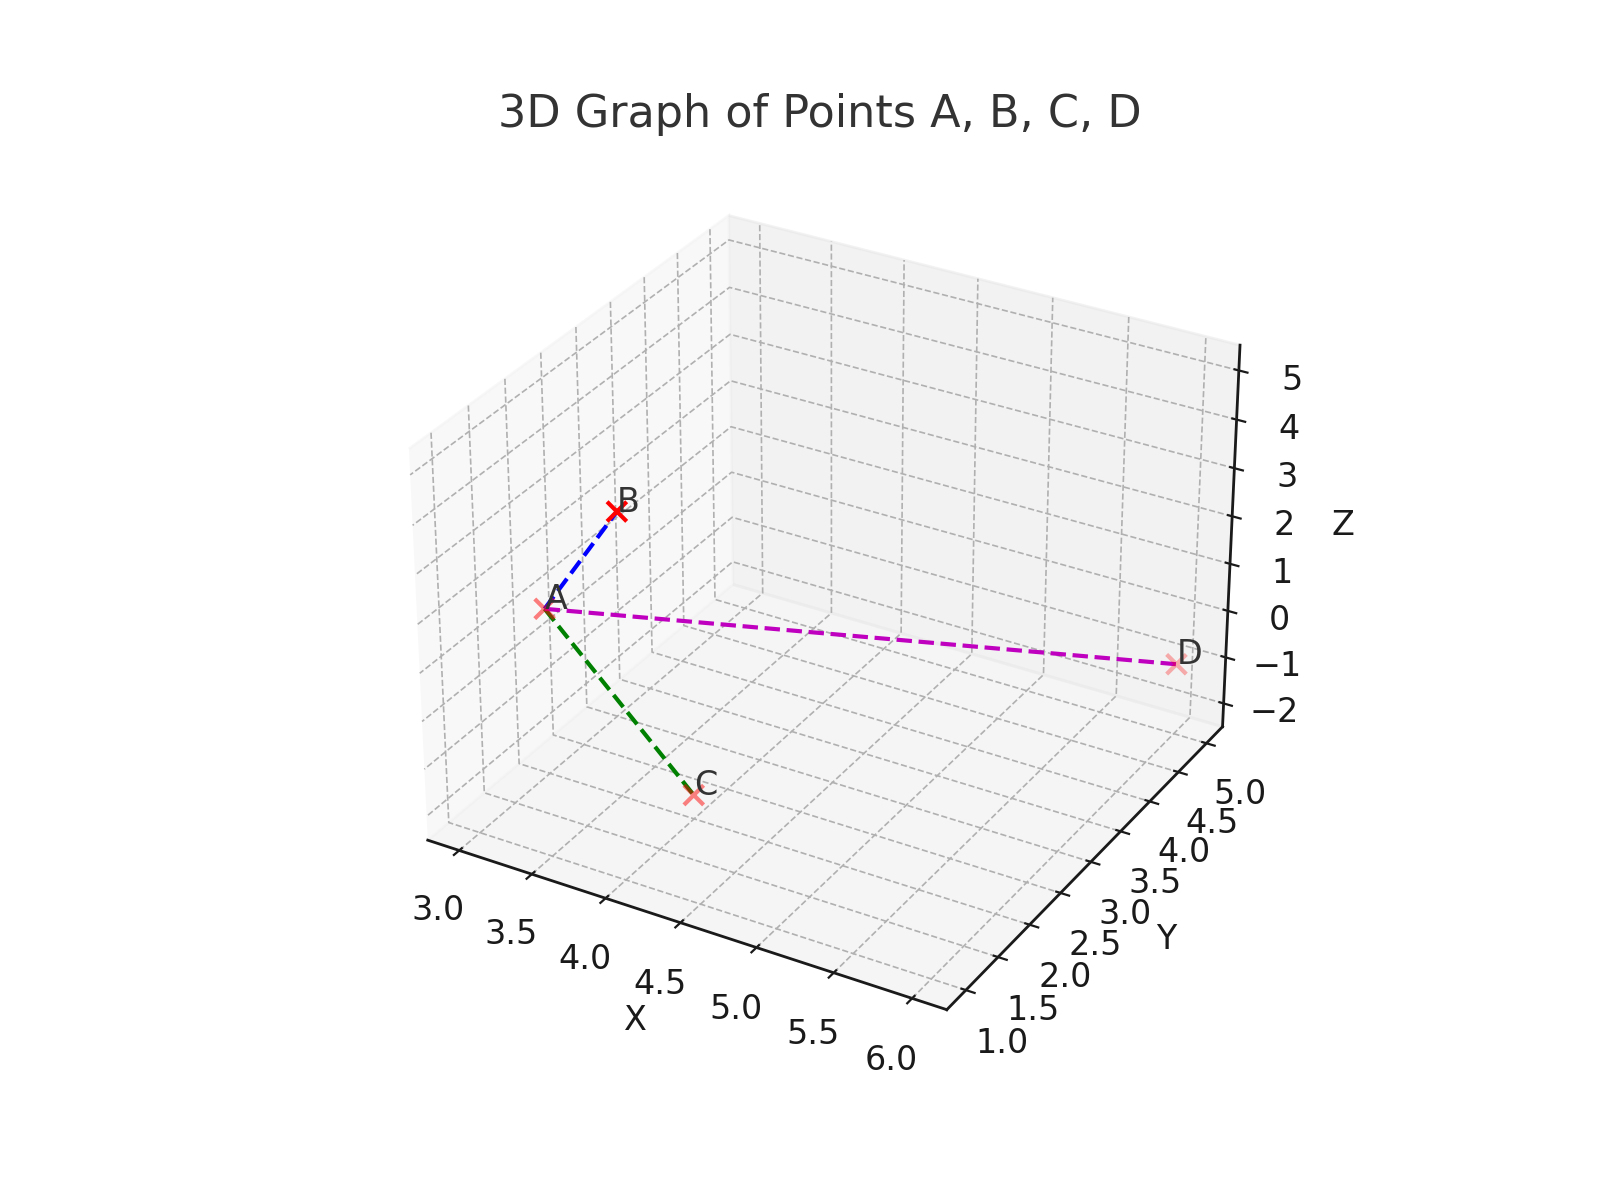
\includegraphics[height=0.5\textheight, keepaspectratio]{figs/3D_points_plot.png}
    \label{figure_1}
\end{figure}
 


\end{document}